\chapter{Preliminaries}
\label{sec:preliminaries}

With the rapid growth in integrated circuit, digital signal processing, and other emerging technologies, people nowadays can easily purchase electronic devices, such as personal computers, laptops, cellular phones, and tablets.  
By utilizing these devices, people can communicate with each other through wireless communication and increase work performance.      
However, any malicious user may misuse these devices and launch serious attack to make illegal profit, such as identity stealing or password cracking on a bank account.
Therefore, it is essential to develop robust methods to solve the identity problems.
With the rapid growth in integrated circuit, digital signal processing, and other emerging technologies, people nowadays can easily purchase electronic devices, such as personal computers, laptops, cellular phones, and tablets.  
By utilizing these devices, people can communicate with each other through wireless communication and increase work performance.      
However, any malicious user may misuse these devices and launch serious attack to make illegal profit, such as identity stealing or password cracking on a bank account.
Therefore, it is essential to develop robust methods to solve the identity problems.
With the rapid growth in integrated circuit, digital signal processing, and other emerging technologies, people nowadays can easily purchase electronic devices, such as personal computers, laptops, cellular phones, and tablets.  
By utilizing these devices, people can communicate with each other through wireless communication and increase work performance.      
However, any malicious user may misuse these devices and launch serious attack to make illegal profit, such as identity stealing or password cracking on a bank account.
Therefore, it is essential to develop robust methods to solve the identity problems, as shown in
~\ref{fig:PHI}.

\begin{figure}[t!]
  \begin{center}
    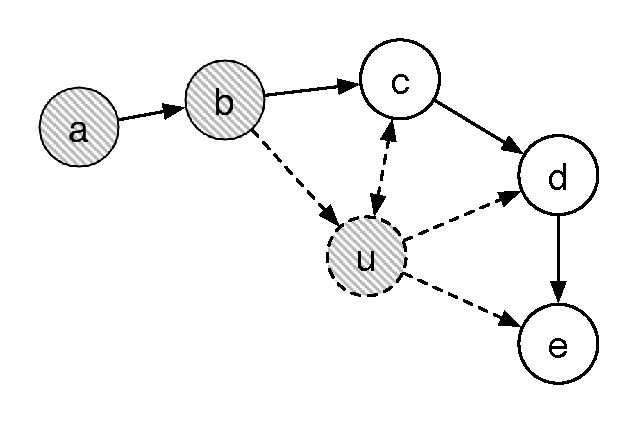
\includegraphics[width=1.0\textwidth]{figures/dyna_rm.eps}
    \caption{The diagram of ``prototypical PHI query''} 
    \label{fig:PHI}
  \end{center}
\end{figure}